\documentclass[pdf]{beamer}

\RequirePackage[utf8]{inputenc}
\RequirePackage[T1]{fontenc}
\RequirePackage{lmodern}

% for speaker notes etc
\RequirePackage{pgfpages}
\setbeameroption{show notes on second screen}
%\setbeameroption{show only notes}
\setbeamercolor{note page}{bg=white}
\setbeamercolor{note title}{bg=white!90!black, fg=black}
\setbeamercolor{note date}{parent=note title}

\beamertemplatenavigationsymbolsempty
\AtBeginSection[]{
    \begin{frame}
        \vfill
        \centering
        \begin{beamercolorbox}[sep=8pt,center,shadow=true,rounded=true]{title}
            \usebeamerfont{title}\insertsectionhead\par%
        \end{beamercolorbox}
        \vfill
    \end{frame}
}

\RequirePackage{listings}
\lstset{escapeinside={<@}{@>}}
\lstset{basicstyle=\ttfamily}
\lstset{moredelim=**[is][\color{red}]{@}{@}}

\RequirePackage{dirtree}
\RequirePackage{csquotes}

\RequirePackage{listings}
% use monospaced fonts in listings
\lstset{basicstyle=\ttfamily}

\mode<presentation>{}

\title{Building C++-Python libraries}
\subtitle{}
\author{Jørgen Kvalsvik <jokva@equinor.com>}
\titlegraphic{
\includegraphics[width=0.33\textwidth]{equinor-red.eps}}

\begin{document}
\maketitle

\begin{frame}{Outline}
    \tableofcontents

    \note{
        \begin{itemize}
            \item something python api for users
        \end{itemize}
    }
\end{frame}

\begin{frame}{Types of Python}
    \begin{itemize}
        \item Pure python
        \item Impure Python (non-python code behind CPython API)
        \item Thin library wrappers
        \item Fat library wrappers
    \end{itemize}

    \note{
        \begin{itemize}
            \item Pure python is what we want out downstream users to do
            \item Impure python is almost indistinguishable from pure python:
                  Numpy and chunks of the python standard library are good
                  examples.
            \item Thin wrappers rely on some system provided library and
                  provide an entry point from Python. Ctypes is often use for
                  this - fire, wait, and parse the output
            \item Rely on larger, often system-wide external libraries, but do
                  more than just provide an entry point - sophisticated I/O,
                  manipulation of state, and rich access to library
                  functionality. Difference between this and impure python is
                  that numpy's backend is only available in python, contrary to
                  say python-BLAS
        \end{itemize}
        We'll focus on impure and fat library.
    }
\end{frame}

\begin{frame}{A goal}
    python3 -m pip install pkg
\end{frame}

\begin{frame}{pip install}
    What does pip install do?

    \begin{enumerate}
        \item Looks up the package name in an \emph{index}
        \item Determines if the package is installable on this system
        \item Fetches the package
        \item Extracts the contents to the right site-package directory
    \end{enumerate}
\end{frame}

\begin{frame}
    \begin{center}
    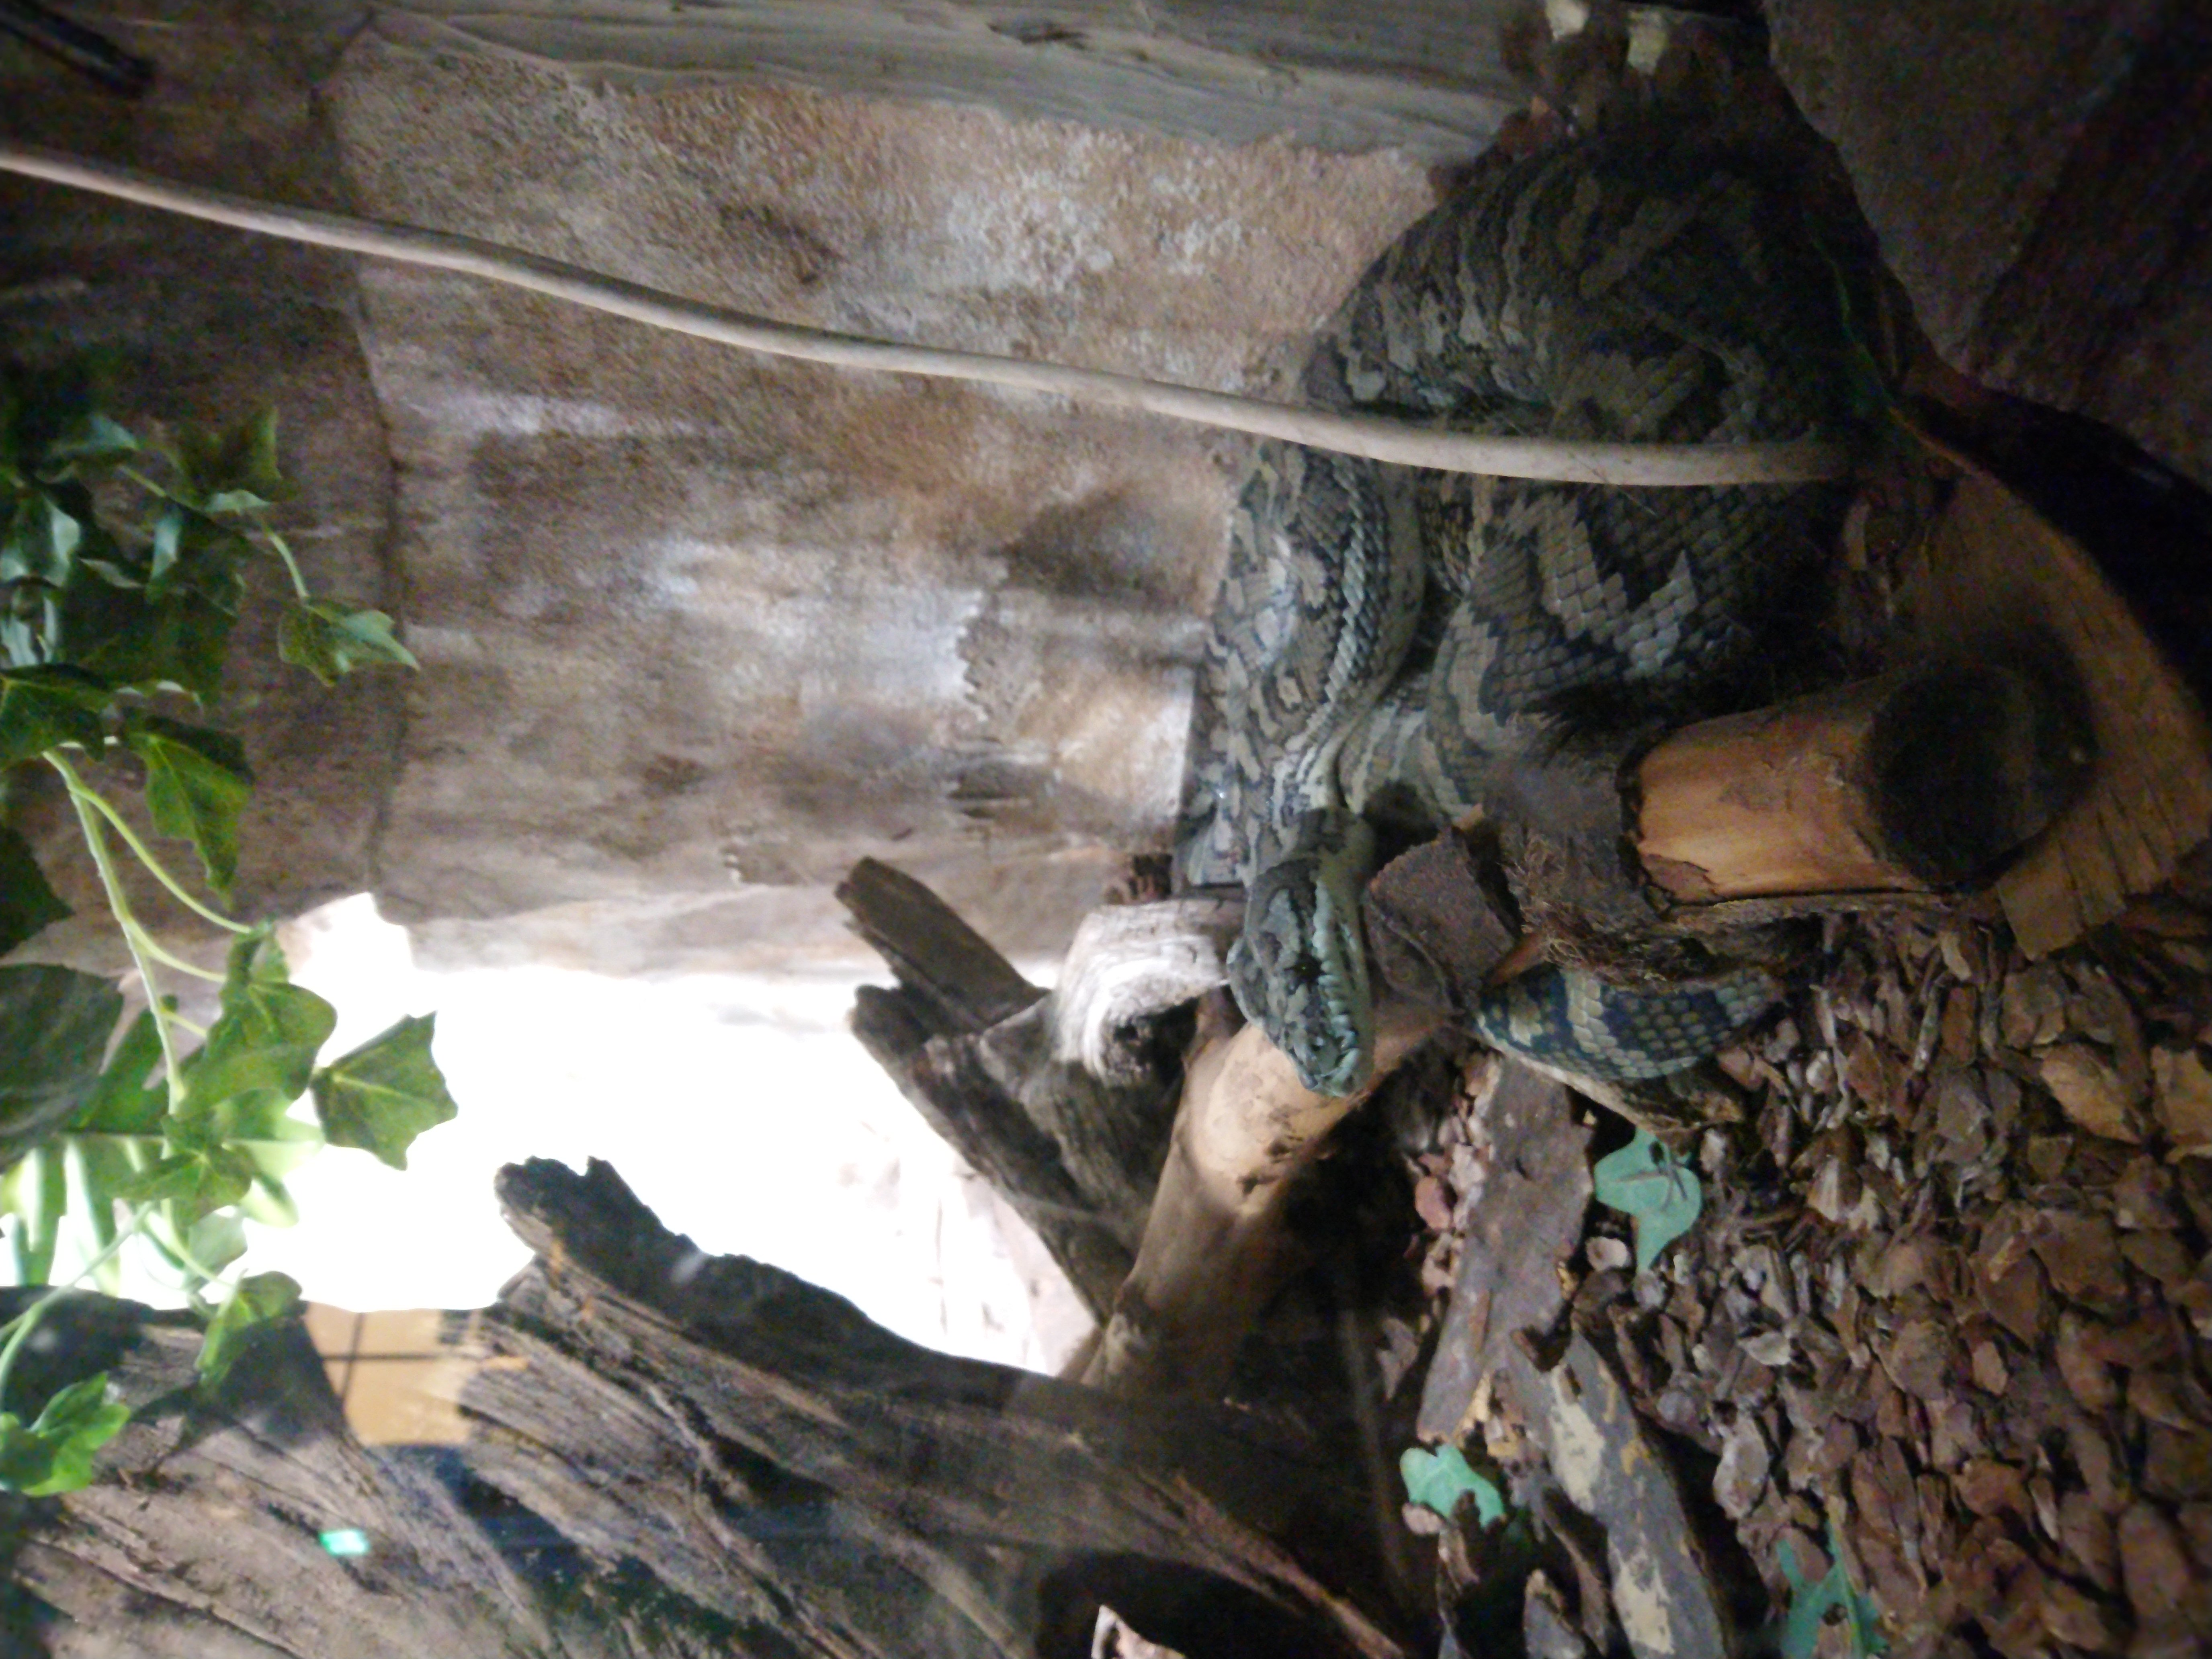
\includegraphics[keepaspectratio, height = 0.9\textheight]{snake.jpg}
    \end{center}
    \note {
        This is a Python package
    }
\end{frame}

\begin{frame}{\emph{Building} interpreted packages 1/2}
    Python packages are just source code, parsed and interpreted on-the-fly

    \note{
        \begin{itemize}
            \item We still talk about \emph{building} packages even though it's
                  a glorified directory copy
            \item To shed some light on it, let's look at the internals of your
                  run-of-the-mill python project
        \end{itemize}
    }
\end{frame}

\begin{frame}{Directory layout 1/3}
    \dirtree{%
        .1 project/.
        .2 README.rst.
        .2 LICENSE.
        .2 setup.py.
        .2 requirements.txt.
        .2 package/.
        .3 {\_\_}init{\_\_}.py.
        .3 core.py.
        .3 helpers.py.
        .2 docs/.
        .3 conf.py.
        .3 index.rst.
        .2 tests/.
        .3 test{\_}basic.py.
        .3 test{\_}advanced.py.
    }

    {\tiny https://www.kennethreitz.org/essays/repository-structure-and-python}

    {\tiny https://docs.python-guide.org/writing/structure}
    \note{
        \begin{itemize}
            \item This is a source tree listing, a git checkout or similar
            \item Building this package is essentially just copying the
                  package/ directory to the correct python/site-packages
            \item Sometimes you want to do some pre-processing to source files,
                  pre-set variables depending on system, bundle data files etc
        \end{itemize}
    }
\end{frame}

\begin{frame}{Directory layout 2/3}
    \dirtree{%
        .1 project/.
        .2 README.rst.
        .2 LICENSE.
        .2 setup.py.
        .2 requirements.txt.
        .2 src/.
        .3 package/.
        .4 {\_\_}init{\_\_}.py.
        .4 core.py.
        .4 helpers.py.
        .2 docs/.
        .3 conf.py.
        .3 index.rst.
        .2 tests/.
        .3 test{\_}basic.py.
        .3 test{\_}advanced.py.
    }

    \note{
        \begin{itemize}
            \item Notice the src/ folder
            \item Can have multiple packages in the same tree
            \item Has a few benefits, such as no implicit import of source code
        \end{itemize}
    }
\end{frame}

\begin{frame}{Directory layout 3/3}
    \dirtree{%
        .1 site-packages/.
        .2 my-package/.
        .3 {\_\_}init{\_\_}.py.
        .3 core.py.
        .3 helpers.py.
        .2 numpy/.
        .2 pandas/.
        .2 minisat/.
    }

    \note{
        \begin{itemize}
            \item Both the previous examples, when built and install, end up
                  like this
        \end{itemize}
    }
\end{frame}

\begin{frame}{\emph{Building} interpreted packages 2/2}
    Building is the transformation from a source-tree to something predictably
    laid out in site-packages

    \note{
        \begin{itemize}
            \item For this, \emph{if} you conform to a common project layout,
                  python tooling works reasonably well.
            \item How did we get here?
        \end{itemize}
    }
\end{frame}

\begin{frame}{Some history}
    
\includegraphics[width=\textwidth]{pantheon.jpeg}
    \note{
        \begin{itemize}
            \item Anyone know what this is?
            \item Important to understand how we got here
        \end{itemize}
    }
\end{frame}


\begin{frame}{Some history}
    \begin{description}
        \item [Late 90s] Python wanted something like CPAN
        \item [2000] Distutils released for Python 1.6 standard library
        \item [2003] PyPI is online, distutils can create package metadata
        \item [2008] Setuptools extends and supersedes distutils, pip builds on it
    \end{description}

    \note{
        \emph{Read the list}: standard library is where modules go to die
        \begin{itemize}
            \item Notice \emph{everything builds on}
            \item Setup written for distutils generally work with setuptools,
                  strong backwards compatibility. This also means a lot of
                  legacy
            \item Distutils came with infrastructure for building C code
            \item Feels much intended for building Python extensions, using the
                  same compiler that built Python.
            \item This is terrible on Windows where dealing with compilers is a
                  pain
            \item Uses homegrown compiler abstraction and option dispatch
                  interface. No robust feature discovery, a C build-system but
                  not really
            \item Building pollutes source tree
            \item Let's start building a package
        \end{itemize}
    }
\end{frame}

\begin{frame}[fragile]{setuptools}
    \lstinputlisting{my-package/setuptools-pure.py}

    \note{
        \begin{itemize}
            \item This is for a pure python package
            \item It's quite minimal, setuptools support a wide range of keys
                  and metadata. It can figure some things out, since our
                  project is "standard layout".
            \item Let's add some native code, a C extension
        \end{itemize}
    }
\end{frame}

\begin{frame}[fragile]{setuptools}
    \lstinputlisting{my-package/my_package/math/math.c}
\end{frame}

\begin{frame}[fragile]{setuptools}
    \lstinputlisting{my-package/setuptools-ext.py}
\end{frame}

\begin{frame}[fragile]{setuptools + extension}
    \begin{lstlisting}
>>> import my_package
>>> my_package.math.add(1, 2)
3
    \end{lstlisting}
    \note {
        \begin{itemize}
            \item This extension is, of course, trivial
            \item Let's spice it up and use C++11
        \end{itemize}
    }
\end{frame}

\begin{frame}[fragile]{setuptools}
    \lstinputlisting{my-package/my_package/math/math11.cpp}
    \note{
        \begin{itemize}
            \item This now fails on gcc < 6.0, because C++98 was still the
                  default
            \item Of course it's still valid C++, so it just needs the option
        \end{itemize}
    }
\end{frame}

\begin{frame}[fragile]{setuptools}
    \lstinputlisting{my-package/setuptools-ext11.py}

    \note{
        \begin{itemize}
            \item Ok good, so this builds... on linux
            \item MSVC doesn't understand this flag
            \item So now our script needs to detect compiler and only set the
                  flag on gcc
            \item ... until we also want to build with clang
            \item If you've ever built C++ for multiple platforms or even
                  different computers you see how this can get problematic fast
            \item Honestly, setup.py-files that do more than setup() and are
                  pure python tend to be low-effort, buggy, \emph{works on my
                  machine} solutions
            \item So now, we give up
        \end{itemize}
    }
\end{frame}

\begin{frame}[fragile]{Building native code}
    The struggle of binary libraries

    \begin{itemize}
        \item Multiple compilers with different flags
        \item Compiler versions
        \item Multiple available compilers
        \item Platform-specific options
        \item Configuration-specific options, e.g. \verb|USE_BLAS|
        \item Feature detection
        \item Build and runtime dependencies
        \item Binary compatibility
    \end{itemize}

    \note{
        \emph{Read list}
        \begin{itemize}
            \item The experience compiling and developing native extensions is
                  terrible
            \item Setuptools has virtually nothing to help you here, boils down
                  to manually implementing half of cmake
            \item The development story is quite bad too
            \item People end up hard-coding links to /opt/local/lib64, I can't
                  blame them
            \item Since setup.py implements build, install, test commands,
                  custom option commands are difficult or clumsy
        \end{itemize}
    }
\end{frame}

\begin{frame}{Developing native code}
    \begin{itemize}
        \item Changes in headers aren't detected, and the module isn't
              recompiled - not great with templates
        \item Designed for distribution, not development
        \item Setuptools assumes it controls the world, so it pollutes source
              trees. Not cool when python support is a sub project
    \end{itemize}

    \note{
        \begin{itemize}
            \item Overall, setuptools does a poor job of tracking file ->
                  compiled object dependencies
            \item Not designing for live development of C based modules is
                  fine, they weren't aiming to build a C build system. But most
                  time is spent is development (by me), and having parallel
                  development and build systems suck
        \end{itemize}
    }
\end{frame}

\begin{frame}{Is paradise lost?}
    \begin{center}
    
\includegraphics[keepaspectratio, height = 0.8\textheight]{fall-of-lucifer.jpg}
    \end{center}
    \note{
        \begin{itemize}
            \item The talk name did hint of a solution
            \item A lot of installed stuff is happy to hard-code path to python
                exe + libs
        \end{itemize}
    }
\end{frame}

\begin{frame}{Enter scikit-build}
    \begin{displayquote}
        The scikit-build package is fundamentally just glue between the
        setuptools Python module and CMake
    \end{displayquote}
    - scikit-build readme

    \note{
        \begin{itemize}
            \item Briefly, it automates building C++ with cmake, and automates
                  dealing with python flags, layout, options.
            \item It adresses most of the shortcomings with setuptools for
                  extensions
            \item For distribution: feature autodiscovery, compiler config,
                  dependency configuration etc
            \item For development: easy debug/release builds, file-object
                  dependency tracking, incremental builds
            \item Setuptools does what setuptools can (build python), cmake
                  does what cmake does
        \end{itemize}
    }
\end{frame}

\begin{frame}[fragile]{CMake}
    cmake gives us:
    \begin{itemize}
        \item \verb|find_package|
        \item \verb|target_link_libraries|
        \item \verb|set(CMAKE_CXX_STANDARD)|
        \item \verb|if (MSVC)|
    \end{itemize}

    \note{
        \begin{itemize}
            \item Hate it or love it, cmake is pretty good at what it does
            \item It's reasonably easy to set options, deal with compiler
                  differences in cmake
            \item When you have third-party dependencies that provide
                  cmake-config or similar, you can easily get them from inside
                  the python extension with find-package
            \item cmake is pretty good at dealing with platform differences
        \end{itemize}
    }
\end{frame}

\begin{frame}[fragile]{scikit-build}
    \lstinputlisting{my-package/CMakeLists.txt}
\end{frame}

\begin{frame}[fragile]{Intermezzo: automate everything}

    \verb|make -j8 && ctest --output-on-failure|

    \note{
        \begin{itemize}
            \item This command is really what I mostly do during development
            \item From a clean checkout, running cmake and then this is
                  sufficient
            \item It builds the core libraries, some applications, the python
                  extension, the python library, and docs if enabled
            \item And runs the tests, across all languages
            \item It uses setup.py to run the python build system, python
                  doesn't really know that it's not the main driver. This is
                  the fat wrapper from before
            \item Now, assuming the impure python, where python is the only
                  player [next slide]
        \end{itemize}
    }
\end{frame}

\begin{frame}[fragile]{setup.py}
    \begin{verbatim}
python3 setup.py build
python3 setup.py test
    \end{verbatim}

    \note{
        \begin{itemize}
            \item This is what we want to run
            \item Let's look at the code needed to drive this
        \end{itemize}
    }
\end{frame}

\begin{frame}[fragile]{setup.py}
    \begin{lstlisting}
import skbuild
skbuild.setup(
    name = 'pkg',
    packages = [
        'pkg',
        'pkg.module',
    ],
    install_requires = [
        'numpy',
    ],
    cmake_args = [
    ],
)
    \end{lstlisting}

    \note{
        \begin{itemize}
            \item \emph{Read slowly}
            \item scikit-build adds a few extra keys and some extra behaviour to
                  setuptools.setup
            \item It implicitly looks for a CMakeLists.txt in the root dir
        \end{itemize}
    }
\end{frame}

\begin{frame}[fragile]{CMakeLists.txt}
    \begin{lstlisting}[basicstyle=\ttfamily\scriptsize]
cmake_minimum_required(VERSION 3.5.0)
project(extension LANGUAGES C CXX)
set(CMAKE_CXX_STANDARD 11)

find_package(PythonExtensions REQUIRED)
find_package(package REQUIRED)

add_library(core MODULE src/core.cpp)
python_extension_module(core)
target_link_libraries(core package::lib)
if (MSVC)
    target_compile_options(core PRIVATE /EHsc)
endif ()

install(TARGETS core LIBRARY DESTINATION package)
    \end{lstlisting}

    \note{
        \begin{itemize}
            \item This is really it. It works quite well, and the maintainers
                  are helpful
            \item It's still not perfect, obviously, but it is a huge leap
                  forward from setuptools and setuptools "abstractions"
            \item Building correctly is a prerequisite for redistributable
                  packages, wheels. We'll get to that later
        \end{itemize}
    }
\end{frame}

\begin{frame}[fragile]{Integration with cmake}
    \begin{lstlisting}[basicstyle=\ttfamily\scriptsize]
add_custom_target(
    dlisio-python ALL
    SOURCES ${setup.py}
    DEPENDS ${setup.py}
    VERBATIM
    WORKING_DIRECTORY ${CMAKE_CURRENT_SOURCE_DIR}
    COMMAND ${python} ${setup.py}
        build_ext --inplace
        build # setup.py build args
            --cmake-executable ${CMAKE_COMMAND}
            --generator ${CMAKE_GENERATOR}
            ${DLISIO_PYTHON_BUILD_TYPE}
        -- # scikit-build cmake args
            -Ddlisio_DIR=${DLISIO_LIB_BINARY_DIR}
            -DCMAKE_INSTALL_RPATH_USE_LINK_PATH=ON
            -DCMAKE_INSTALL_RPATH=$<TARGET_FILE_DIR:dlisio>
            -DCMAKE_INSTALL_NAME_DIR=$<TARGET_FILE_DIR:dlisio>
)
add_dependencies(dlisio-python dlisio)
    \end{lstlisting}

\note{
    \begin{itemize}
        \item This is taken from dlisio
        \item If you're not familiar with cmake or custom targets, this might
              be confusing, but it makes so the python lib behaves like any
              other C++ lib from cmake's perspective
        \item Build in-place so that tests can be run directly on the source
              tree. Setuptools pollutes this directory anyway, so we're not
              really that much worse off - this is the path of least resistance
        \item Scikit-build builds for different python versions in different
              dirs, so they coexist ok
        \item setup.py tracks the python dependencies - the drawback is even
              though there's nothing to do we still must run the seutp.py file.
              This is somewhat slow, but an acceptable tradeoff
    \end{itemize}
}
\end{frame}

\begin{frame}[fragile]{Building wheels}
    The python packaging format is the \emph{wheel}

    \begin{block}{}
        \begin{itemize}
            \item setup.py can build with \verb|setup.py bdist_wheel|
            \item Relies on naming to distinguish package flavours
            \item Can both be pure python or include binary components
            \item pip resolves these names from the host system
        \end{itemize}
    \end{block}

    \begin{block}{From PyPI}
        \begin{verbatim}
segyio-1.8.6-cp37-cp37m-manylinux1_x86_64.whl (87.5 kB)
segyio-1.8.6-cp37-cp37m-win32.whl (83.4 kB)
segyio-1.8.6-cp37-cp37m-win_amd64.whl (89.7 kB)
        \end{verbatim}
    \end{block}

    \note{
        \begin{itemize}
            \item \emph{Read list on screen}
            \item OS X was omitted because it's quite long, but follows the
                  same pattern
            \item The manylinux image is specified by the PyPA, basically the
                  oldest libc + supporting libs they could use (RHEL5)
        \end{itemize}
    }
\end{frame}

\begin{frame}[fragile]{Intermezzo: building wheel on Debian 10 (Buster)}
    \verb|segyio-1.8.6-cp37-cp37m-linux_x86_64.whl|
    \note{
        \begin{itemize}
            \item Notice it says linux, not manylinux. Pip will not fetch
                  packages with this tag, but you can install it at your own
                  machine
            \item Which happens to be what we need to build wheels pip can use
        \end{itemize}
    }
\end{frame}

\begin{frame}
    Problem: I have no machine running Windows
\end{frame}

\begin{frame}
    Problem: I have no machine running Red Hat 5

    \note{
        We'll solve these problems in a bit
    }
\end{frame}

\begin{frame}{Build automation}
    \begin{center}
    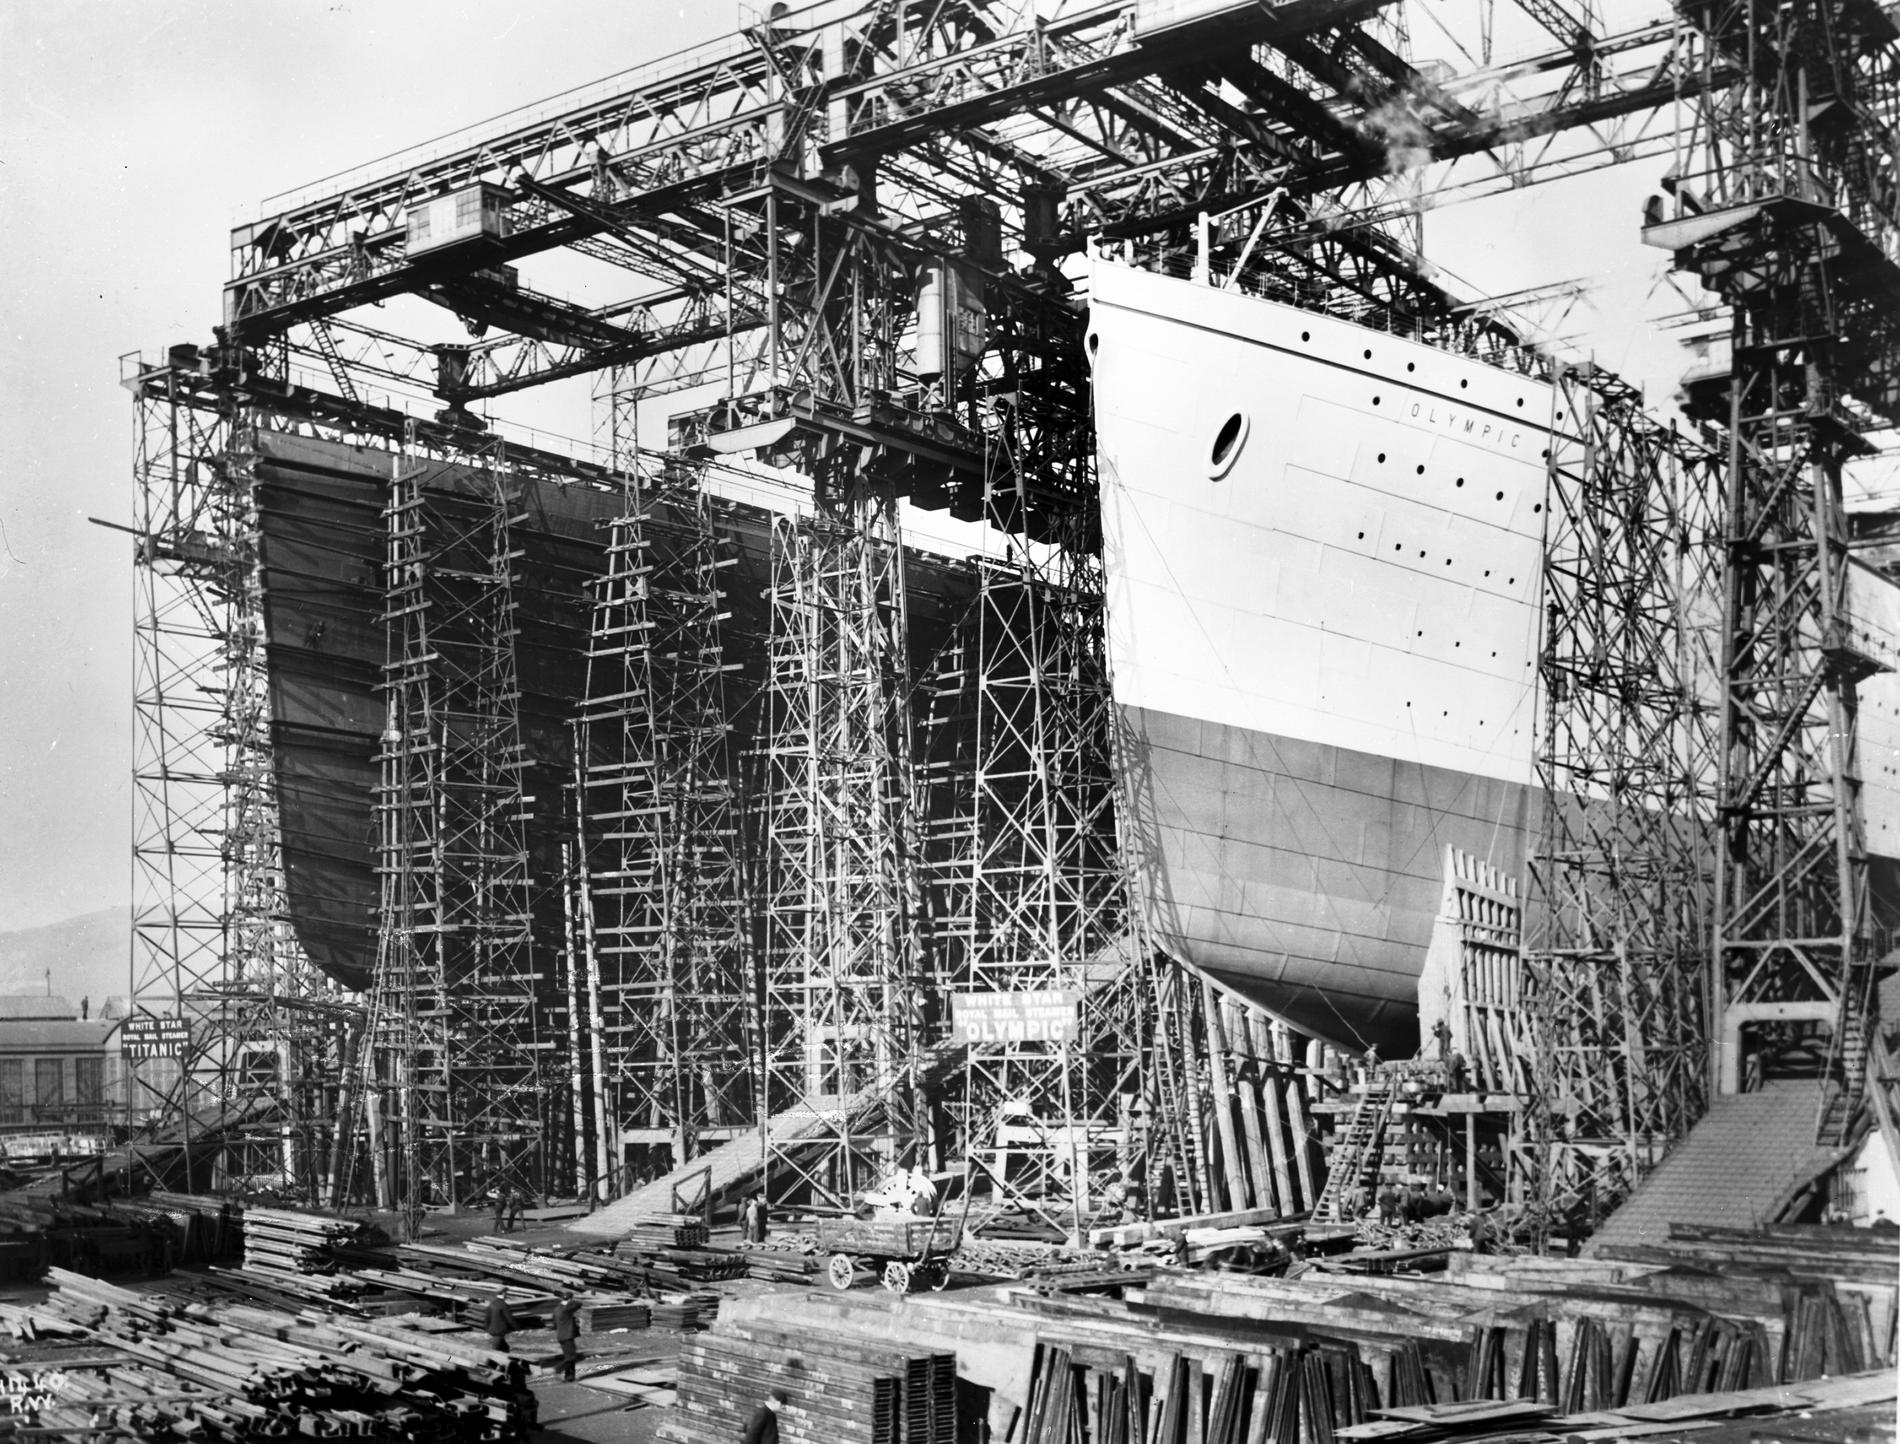
\includegraphics[keepaspectratio, height = 0.8\textheight]{olympic-titanic.jpg}
    \end{center}
    \note{
        \begin{itemize}
            \item Ok, so now we can reasonably easy build and develop on the
                  developer machine
            \item That's still not enough - want to test multiple versions,
                  compilers, operating systems
            \item Most of our projects \emph{are} in fact used across multiple
                  systems, but even if that wasn't the case I'd still insist on
                  it
            \item Targeting different systems improves robustness and
                  correctness - if platforms differ it's because of latent bugs
            \item Also helps the contributor experience - contributors don't
                  have to set up massive rigs, and are generally terrible at
                  running and writing tests
        \end{itemize}
    }
\end{frame}

\begin{frame}{Build automation}
    \begin{block}{Lesson}
        Things not done automatically will not be done
    \end{block}
    \note{
        \begin{itemize}
            \item We use multiple - travis, circle, appveyor. These are what we
                  use rigt now, but like with code there's always maintenance,
                  considering other providers etc
            \item We use them to test on all platforms, multiple versions
            \item Run on every pull request before merge, and all HEADs on
                  master
            \item We also use it for building and releasing packages
            \item CI is scripts + machine definition + triggers
            \item Perfect usecase for obsolete systems like RHEL5 and Windows
            \item So what does it look like?
        \end{itemize}
    }
\end{frame}

\begin{frame}[fragile]{Build automation}
    \begin{lstlisting}[basicstyle=\ttfamily\scriptsize]
commands:
  cmake_build:
    steps:
      - run:
          name: configure
          command: |
            mkdir build && cd build
            cmake -DBUILD_SHARED_LIBS=ON \
                  -DPYTHON_EXECUTABLE=`which python3` \
                  ..
      - run:
          name: build, install, test
          command: |
            cmake --build build --target install
            cd build && ctest --output-on-failure

jobs:
  gcc:
    docker:
      - image: debian:stable
    steps:
      - checkout
      - install_build_deps
      - cmake_build
    \end{lstlisting}
    \note{
        \begin{itemize}
            \item This is for one of our CircleCI configs (we have about 10)
                  and abbreviated slightly for slide purposes
            \item The other services are configured similarly
            \item Usually it's a yaml with special keys and inline scripts -
                  they're all reasonably well documented
        \end{itemize}
    }
\end{frame}

\begin{frame}{Build automation}
    % Workflow pictorial
    fork -> PR -> green checkmark -> merge -> deploy
\end{frame}

\begin{frame}[fragile]{Deploy}
\begin{lstlisting}
deploy:
    - provider: pypi
      skip_cleanup: true
      skip_upload_docs: true
      skip_existing: true
      user: statoil-travis
      distributions: --skip-cmake build sdist
      password:
        secure: encrypted-key
      on:
        tags: true
\end{lstlisting}

    \note{
        \begin{itemize}
            \item Whenever a new tag is pushed, which also happens with the
                  release-feature on github, this runs at the end of the job
            \item It takes the freshly-built package and uploads it to pypi
            \item That means the only thing done to publish new releases is to
                  create a new tag
            \item Means tags are the authority and single source of truth
            \item TODO: Diagram of this flow?
        \end{itemize}
    }
\end{frame}

\end{document}
